\documentclass[notitlepage]{report}
\usepackage[margin=1in]{geometry} 
\usepackage{amsmath,amsthm,amssymb,amsfonts}
\usepackage{tabto}
\usepackage[yyyymmdd]{datetime}		% Date Formatting
\renewcommand{\dateseparator}{--}	% Date Formatting
\usepackage{arydshln} 				% \hdashline and \cdashline
\newcommand*{\tempb}{\multicolumn{1}{:c}{}} % Used for block matrices

% For clickable TOC
\usepackage{hyperref}
\hypersetup{
	colorlinks,
	citecolor=black,
	filecolor=black,
	linkcolor=black,
	urlcolor=black
}

% Custom Section Types
\theoremstyle{plain} % italics
\newtheorem*{thrm}{Theorem}
\newtheorem*{lemma}{Lemma}
\theoremstyle{definition} % normal type
\newtheorem*{ex}{Example}
\newtheorem*{defn}{Definition}
\newtheorem*{result}{Result}
\theoremstyle{plain} % italics

% For circled text
\usepackage{tikz}
\newcommand*\circled[1]{\tikz[baseline=(char.base)]{
            \node[shape=circle,draw,inner sep=0.8pt] (char) {#1};}}

% For equation system alignment
\usepackage{systeme,mathtools}
% Usage:
%	\[
%	\sysdelim.\}\systeme{
%	3z +y = 10,
%	x + y +  z = 6,
%	3y - z = 13}

\newenvironment{problem}[2][Problem]{\begin{trivlist}
\item[\hskip \labelsep {\bfseries #1}\hskip \labelsep {\bfseries #2.}]}{\end{trivlist}}
%If you want to title your bold things something different just make another thing exactly like this but replace "problem" with the name of the thing you want, like theorem or lemma or whatever
 
%used for matrix vertical line
\makeatletter
\renewcommand*\env@matrix[1][*\c@MaxMatrixCols c]{%
  \hskip -\arraycolsep
  \let\@ifnextchar\new@ifnextchar
  \array{#1}}
\makeatother 
 
% Change chapter numbering
\newcommand{\mychapter}[2]{
	\setcounter{chapter}{#1}
	\setcounter{section}{0}
	\chapter*{#2}
	\addcontentsline{toc}{chapter}{#2}
}
\begin{titlepage}
\title{Final Exam}
\author{Bryan Greener}
\date{2018-06-23}
\end{titlepage}


\begin{document}
% BUILD TOC
%\tableofcontents{}
\maketitle
\begin{enumerate}
\item How is a typical model neuron in a Neural Network:
	\begin{enumerate}
	\item Like a biological neuron?
	\medskip\\
		Our understanding on biological neurons is that they are transmitters that receive various signals, from other neurons or from some other form of input, they then perform some action on the electrical signal to modulate it, and finally they pass the updated signal to another neuron or to some other receiver. The neurons used in neural networks are similar in the sense that they receive some number of inputs either from the data source or from previous neurons. They then use an activation function to manipulate the values being passed in. Finally they output this new value and pass it on to the next neuron or to the system output.
	\item Unlike a biological neuron?
	\medskip\\
		Unlike biological neurons, the neural network neurons that we are creating are very isolated. What this means is that they are not aware of the changes being made to neighboring neurons. On top of this, the ANS neurons are limited to working with only the network design that they are given. They do not have any plasticity in terms of changing their neighboring neurons on their own.
	\item Suggest a characteristic inspired by a biological neuron that would add to the learning capability of an Artificial Neural System.
	\medskip\\
		As previously mentioned, biological neurons are influenced by neighboring neurons in ways that we don't fully understand at this point. When we finally understand how and why neurons behave this way, then we can use that feature in our artifical neurons to improve accuracy, functionality, or whatever that grouping improves in biological neural systems.
	\end{enumerate}

\item Gradient Descent
	\begin{enumerate}
	\item Describe gradient descent and how it can guide a learning rule. What is its most basic flaw?
	\medskip\\
		Gradient descent is an algorithm used to locate minima in an n-dimensional loss function. By finding an algorithm's current gradient after plugging inputs into the function, we can take steps down the gradient closer and closer to a minimum in the function which means that our algorithm's error decreases. The biggest problem with gradient descent is that functions don't always have a single minimum value and so it is easy for gradient descent to find a minimum value but this minima is likely not the lowest possible value in the function. This can be remedied using momentum and other algorithms that help to avoid getting stuck in local minima.
	\item Why are sigmoid style activation functions used in backprop?
	\medskip\\
		The sigmoid function and other functions like it are useful for taking input values and normalizing them between two numbers in a non-linear fashion. For example, if you have hundreds of values between 0 and 50 and a single outlier with a value of 100, then the sigmoid function will bring all the values between 0.0 and 1.0 but a value that was previously 50 might be 0.99 now and the outlier of 100 would then be 0.999. This prevents that outlier from affecting the network too much and causing overfitting in the training process.
	\end{enumerate}

\item What is the ''energy'' of a system as in Hopfield nets? How does this global measure guide system dynamics?
\medskip\\
	The term energy used in Hopfield nets is referring to the scalar value representing the cost of the network at a specific timestep. By updating the energy at each timestep to bring it to a lower state, the system will reach its local minima. This is the same as minimizing the error using a cost function in other types of neural networks.
	
\item In the attached paper, consider equation 2.
	\begin{enumerate}
	\item Graph the equation for a very large $T$ and for $T=1$.
	\medskip\\
		To my understanding, equation 2 in the paper (shown below) will behave like a sigmoid function.
		\[ P(S_i = 1) = \dfrac{1}{1+e^{-\frac{\Delta V}{T}}} \]
		Thus our graph is as follows.\\
		\begin{center}
		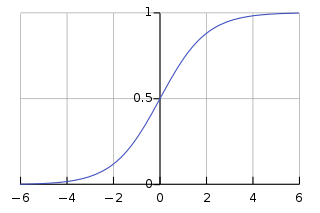
\includegraphics[scale=0.5]{sigmoid.png}
		\end{center}
		Since this function is bounded by $[0,1]$ then $0 \leq f(x) \leq 1$ for all $x\in\mathbb{R}$.
	
	\item Explain why Boltzmann learning causes the system to converge on system states that represent better solutions.
	\medskip\\
		Using simulated annealing allows the network to converge around the global minimum instead of the local minimum in a function. This is because of the nature of the machine resetting its state at each time unit, preventing the machine from reaching a thermal equilibrium.
		
	\item How can stochastic activations avoid the flaw in gradient descent?
	\medskip\\
		By implementing stochastic methods in our networks, we prevent overfitting in the model. This is due to the fact that we are not training on the same set of data in the same order over and over, which would cause the network to ''memorize'' that pattern.
	\end{enumerate}
	
\item One could teach the LSTM algorithm without saying the word 'neural net' \--- simply as a clever algorithm and data structure. But are there essential characteristics that a 'neural network' or 'deep learning' approach bring to AI solutions, if at all?
\medskip\\
	While the LSTM algorithm can be taught purely from a mathematical point of view, I believe that relating it to neural networks allows us to understand the intuition behind what this algorithm is doing. This same statement applies to artificial neural networks in general \-- they can all be taught just with math and statistics. However by explaining how they relate to our brains we can take inspiration from ourselves and develop artificial networks by mimicking nature's design. This allows us to see where we may improve if we hope to make a network that actually 'thinks' more like we do. 
\end{enumerate}

\end{document}
